\documentclass[12pt,prb,aps]{revtex4-1}
\usepackage {amsmath}
\pdfoutput = 1 
\usepackage {graphicx}

\begin{document}

\title{Further drift-magnetohydrodynamic modeling of linear tearing mode dynamics in tokamak plasmas}

\author{R.~Fitzpatrick\,\footnote{rfitzp@utexas.edu}}
\affiliation{Institute for Fusion Studies,  Department of Physics,  University of Texas at Austin,  Austin TX, 78712, USA}

\begin{abstract}
An improved 
\end{abstract}

\maketitle

\section{Introduction}
Tearing modes are slowly growing instabilities of ideally-stable tokamak plasmas that reconnect magnetic field-lines
at various resonant surfaces within the plasma, in the process degrading the plasma confinement.\cite{wes}
If tearing modes gorw to sufficiently large amplitude then they can trigger major disruptions.\cite{wes1}  Tokamak
plasma are observed to be particularly disruption prone when tearing modes {\em lock}\/ (i.e., become stationary in the
laboratory frame) to externally generated, resonant magnetic perturbations.\cite{vries}  

It is well known that single-fluid resistive magnetohydrodynamics (MHD) offers a very poor description of
tearing mode dynamics in tokamak plasmas. 
For instance, the strong {\em diamagnetic}\/ flows present in such plasmas decouple the electron and ion fluid dynamics,
necessitating a two-fluid treatment.\cite{ara} Moreover, resistive-MHD does not take  the important {\em ion sound radius lengthscale}, below which electron and ion dynamics are further decoupled, 
into account.\cite{drake,wal} Previously, Cole \& Fitzpatrick\,\cite{cole} used the four-field model
of Fitzpatrick \& Waelbroeck\,\cite{fw} (which is based on the original four-field model of Hazeltine, et al.\cite{haz}),
to determine the two-fluid response of a linear tearing layer in a tokamak plasma to an externally generated, 
resonant magnetic perturbation. However, the treatment of Cole \& Fitzpatrick failed to take into account the
strong anomalous perpendicular transport of particles and energy present in tokamak plasmas. The
aim of this paper is to correct this deficiency. 

\section{Four-Field Model}

\section*{Acknowledgements}
This research was directly funded by the U.S.\ Department of Energy, Office of Science, Office of Fusion Energy Sciences,  under  contracts DE-FG02-04ER54742 and DE-SC0021156. 

\section*{References}
\begin{thebibliography}{99}\baselineskip 5ex

\bibitem{wes} J.A.~Wesson, Nucl.\ Fusion {\bf 18}, 87 (1978).

\bibitem{wes1} J.A.~Wesson, et al.\ Nucl.\ Fusion {\bf 29}, 641 (1989).

\bibitem{vries} P.C. de Vries, et al.\ Nucl.\ Fusion {\bf 51}, 053018 (2011).

\bibitem{ara} G.~Ara, B.~Basu, B.~Coppi, G.~Laval, M.N.~Rosenbluth, and B.V.~Waddell, Ann.\ Phys.\ (NY) {\bf 112}, 443 (1978).

\bibitem{drake} J.F.~Drake, and Y.C.~Lee, Phys.\ Fluids {\bf 20}, 1341 (1977).

\bibitem{wal} F.L.~Waelbroeck, Phys.\ Plasmas {\bf 10}, 4040 (2003).

\bibitem{cole} A.~Cole, and R.~Fitzpatrick, Phys.\ Plasmas {\bf 13}, 032503 (2006).

\bibitem{fw} R.~Fitzpatrick, and F.L.~Waelbroeck, Phys. Plasmas {\bf 12}, 022307 (2005).

\bibitem{haz} R.D.~Hazeltine, M.~Kotschenreuther, and P.G.~Morrison, Phys.\ Fluids {\bf 28}, 2466 (1985).

\end{thebibliography}

%\begin{figure}
%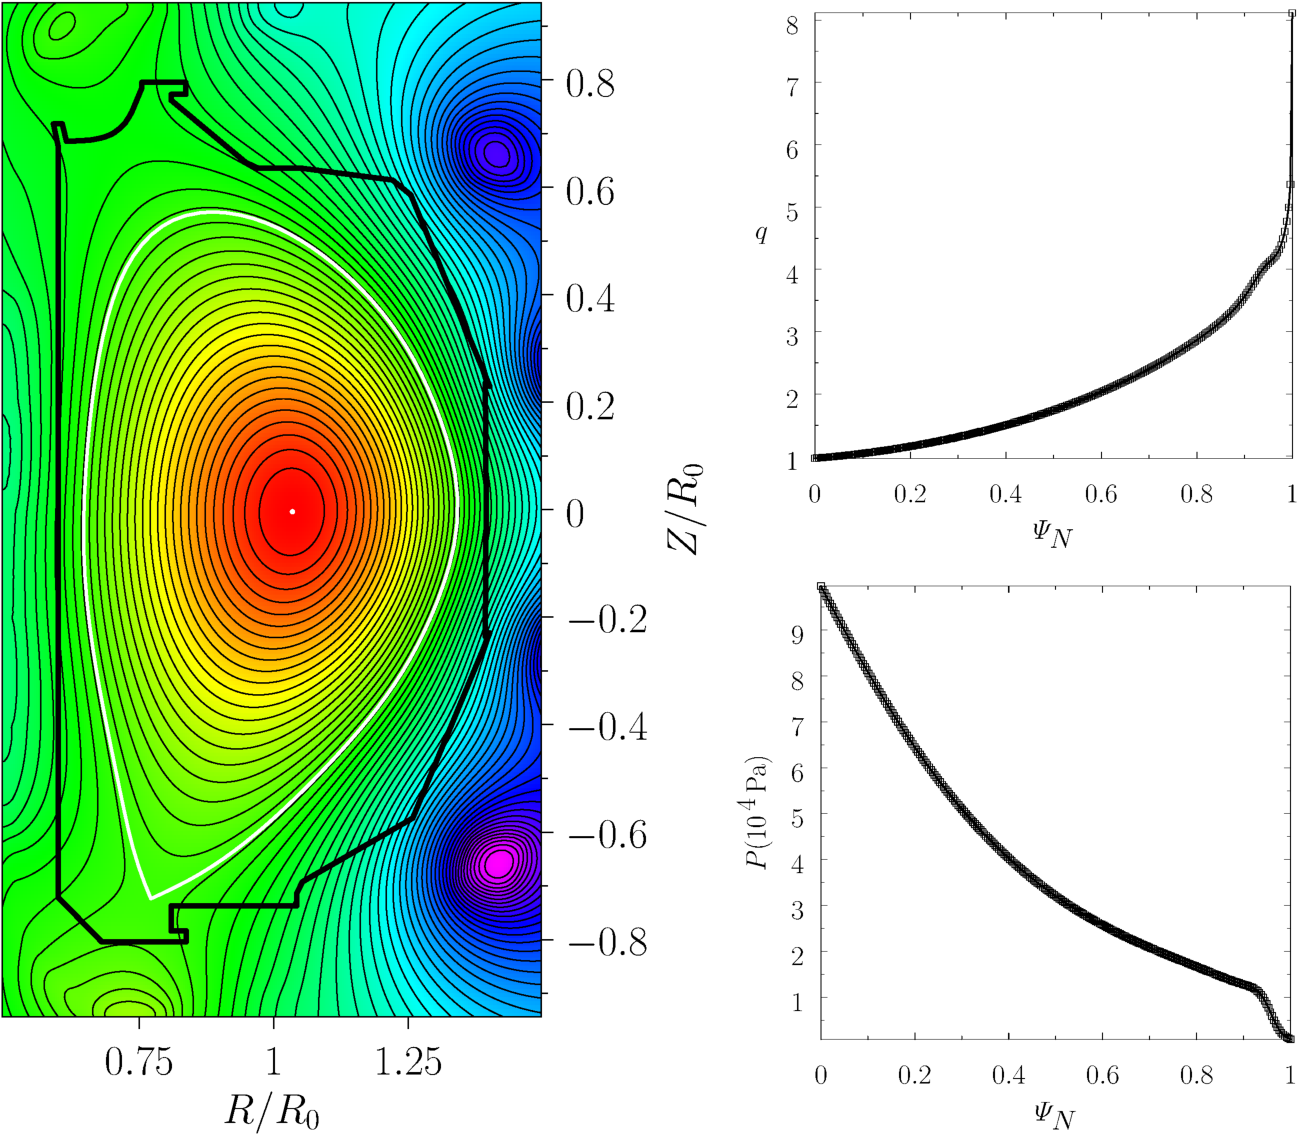
\includegraphics[height=6in]{fig2.pdf}
%\caption{}
%\end{figure}
\end{document}